\documentclass[11pt]{article}

\usepackage[margin=1in]{geometry}
\usepackage{graphicx}
\graphicspath{{./images/}{../images/}{./overleaf_microplastic_project/images/}}
\usepackage{booktabs}
\usepackage{amsmath}
\usepackage[utf8]{inputenc}
\usepackage[T1]{fontenc}
\usepackage{hyperref}
\usepackage{url}
\usepackage{xcolor}
\usepackage{float}
\usepackage{subcaption}
\usepackage{array}

\hypersetup{
  colorlinks=true,
  linkcolor=blue!45!black,
  citecolor=blue!45!black,
  urlcolor=blue!45!black
}

\title{\vspace{-1.5em}Deep Learning Segmentation of Microplastics in Ecological Microscopy Images}

\author{\small
Alex Dils$^{1}$, Jack Spottiswood$^{1}$, Dylan Karmin$^{2}$, Win Cowger$^{3,4}$,\\
David Raymond$^{5}$, Samay Kodige$^{1}$, Rikhil Kokal$^{1}$, Christoph Sad\'ee$^{6}$\\[0.5em]
\footnotesize $^{1}$University of California, Berkeley;
$^{2}$Massachusetts Institute of Technology;
$^{3}$University of California, Riverside;\\
\footnotesize $^{4}$Moore Institute for Plastic Pollution Research;
$^{5}$Dartmouth College;
$^{6}$Stanford University
}

\date{}

\begin{document}
\maketitle

\begin{abstract}
Reliable visual measurement of microplastics in environmental samples remains labor-intensive because particles are small, morphologically diverse, and often embedded in visually cluttered ecological backgrounds. We present a focused semantic segmentation study for pixel-level microplastic masking in microscopy images. The dataset contains 368 labeled laboratory microplastic images, 733 ecological background images, and a locked 97-image ecological microplastic test set. We trained six semantic segmentation architectures under two supervised data regimes: real labeled training images only and real images supplemented with synthetic inpainted ecological context. All completed checkpoints were evaluated on the same held-out ecological test set. The strongest model was SegFormer-B2 trained on real images only, reaching Dice 0.743, mask IoU 0.619, and boundary F1 0.809 on the held-out ecological set. Across models, real-only training achieved higher test performance than real-plus-inpainting training (mean Dice 0.641 vs. 0.444), despite the inpainting condition producing very high validation Dice. These results show that strong segmentation of ecological microplastic microscopy images is feasible, but they also demonstrate that synthetic ecological inpainting can substantially overestimate generalization if judged only on validation data. The study provides a reproducible benchmark, visual evidence, and a practical baseline for segmentation-assisted microplastic image screening.
\end{abstract}

\section{Introduction}

Microplastic contamination is a persistent environmental and public-health concern. Particles occur across marine, freshwater, food, and drinking-water systems, and reliable monitoring depends on workflows that can detect, count, and characterize small particles at scale \cite{geyer2017,ziani2023}. Current analytical pipelines often combine sample preparation, microscopy, expert visual inspection, and chemical confirmation by Fourier-transform infrared spectroscopy or Raman spectroscopy \cite{hidalgo2012,stock2020,primpke2020}. These methods are scientifically grounded but expensive, slow, and difficult to scale across large environmental monitoring programs.

Computer vision can reduce the screening burden by identifying candidate particles in microscopy images before expert review or spectroscopic confirmation. For microplastic analysis, segmentation is particularly valuable because a pixel-level mask supports area, boundary, shape, and morphology measurements. These measurements are difficult to recover from image-level classification or bounding boxes alone. Prior work has shown that deep learning can support microplastic counting, detection, and segmentation in controlled image settings \cite{lorenzo2021,park2022mpnet,shi2022sem,hao2024,yao2025}. Ecological brightfield microscopy remains challenging because microplastics can be transparent, thin, fragmented, or visually similar to sediment, bubbles, fibers, and organic debris.

The central obstacle is generalization. Labeled microplastic microscopy datasets are limited, and laboratory-prepared images often differ from ecological samples. Synthetic image generation is therefore attractive: ecological background images can be combined with known microplastic masks to create additional labeled training examples. However, synthetic data can also introduce artifacts, alter foreground-background statistics, or create validation sets that are easier than real ecological images. A publishable segmentation result must therefore be evaluated on a locked ecological test set rather than on synthetic validation data alone.

This paper reports a focused segmentation experiment using only completed, verified runs. We compare real-only training with real-plus-inpainting training across six semantic segmentation architectures and three random seeds. The goal is to present a concise, journal-ready account of what is currently supported by held-out ecological test results.

\section{Materials and Methods}

\subsection{Image Cohorts}

The study uses three microscopy cohorts with distinct roles (Table~\ref{tab:datasets}). Cohort 1 contains laboratory microplastic images with binary masks and provides the real supervised training source. Cohort 2 contains ecological microscopy backgrounds and provides background context for synthetic inpainting. Cohort 3 contains ecological microplastic images with binary masks and is reserved as the locked held-out test set.

\begin{table}[H]
  \centering
  \caption{Image cohorts used in the focused segmentation study.}
  \label{tab:datasets}
  \small
  \begin{tabular}{p{0.13\textwidth}p{0.25\textwidth}rrp{0.28\textwidth}}
    \toprule
    \textbf{Cohort} & \textbf{Image type} & \textbf{Images} & \textbf{Masks} & \textbf{Role} \\
    \midrule
    Cohort 1 & Laboratory microplastic microscopy & 368 & 368 & Real supervised training source. \\
    Cohort 2 & Ecological microscopy backgrounds & 733 & 0 & Background source for inpainted ecological context. \\
    Cohort 3 & Ecological microplastic microscopy & 97 & 97 & Locked held-out test set. \\
    \bottomrule
  \end{tabular}
\end{table}

Binary masks identify microplastic foreground pixels. Images were resized to \(512 \times 512\) for training and inference; predictions were resized back to original image dimensions before scoring. The Cohort 3 test set was not used for training, validation, threshold selection, prompt selection, or model selection.

\begin{figure}[H]
  \centering
  
\includegraphics[width=0.74\textwidth]{fig_dataset_counts.pdf}
  \caption{Dataset scale. The experiment separates labeled laboratory images, unlabeled ecological backgrounds, and a locked ecological microplastic test set.}
  \label{fig:dataset-counts}
\end{figure}

\subsection{Training Conditions}

We evaluated two completed data regimes. In the real-only condition, models were trained with labeled Cohort 1 images only. In the real-plus-inpainting condition, the same real training images were supplemented with inpainted ecological images generated by inserting transformed Cohort 1 masks into Cohort 2 backgrounds. The retained binary masks were used as segmentation labels for the generated images.

The inpainting arm was included to test whether synthetic ecological context improves generalization. It was not used to tune the Cohort 3 test set, and inpainted images were never included in Cohort 3.

\subsection{Segmentation Models}

Six semantic segmentation architectures were evaluated: U-Net with a ResNet34 encoder, U-Net++ with an EfficientNet-B4 encoder, DeepLabV3+ with a ResNet50 encoder, Feature Pyramid Network with an EfficientNet-B3 encoder, MONAI U-Net, and SegFormer-B2 \cite{ronneberger2015,zhou2018,chen2018,lin2017,xie2021}. Each condition-model pair was trained with seeds 13, 37, and 101, giving 36 semantic checkpoints.

All semantic models were trained with Dice plus binary cross-entropy loss. Training used random flips, translation, crop, shear, and color jitter. The maximum training length was 80 epochs, with early stopping patience of 15 epochs, batch size 8, learning rate \(10^{-4}\), and weight decay \(10^{-5}\). The segmentation threshold was fixed at 0.5 for evaluation.

\subsection{Evaluation Metrics}

The primary test metrics were Dice and mask intersection over union (IoU):
\begin{equation}
\mathrm{Dice} = \frac{2TP}{2TP + FP + FN}, \qquad
\mathrm{IoU} = \frac{TP}{TP + FP + FN}.
\end{equation}
Secondary metrics were precision, recall, boundary F1, and foreground area error. Confidence intervals for top runs were computed by bootstrap resampling over the 97 held-out Cohort 3 images. Validation metrics are reported only to diagnose generalization gaps; Cohort 3 metrics are the primary results.

\section{Results}

\subsection{Held-Out Ecological Test Performance}

The strongest completed checkpoint was SegFormer-B2 trained on real images only with seed 37. It achieved Dice 0.743, IoU 0.619, boundary F1 0.809, precision 0.702, and recall 0.844 on the 97-image ecological test set. The 95\% bootstrap interval was 0.706--0.778 for Dice and 0.580--0.656 for IoU.

\begin{figure}[H]
  \centering
  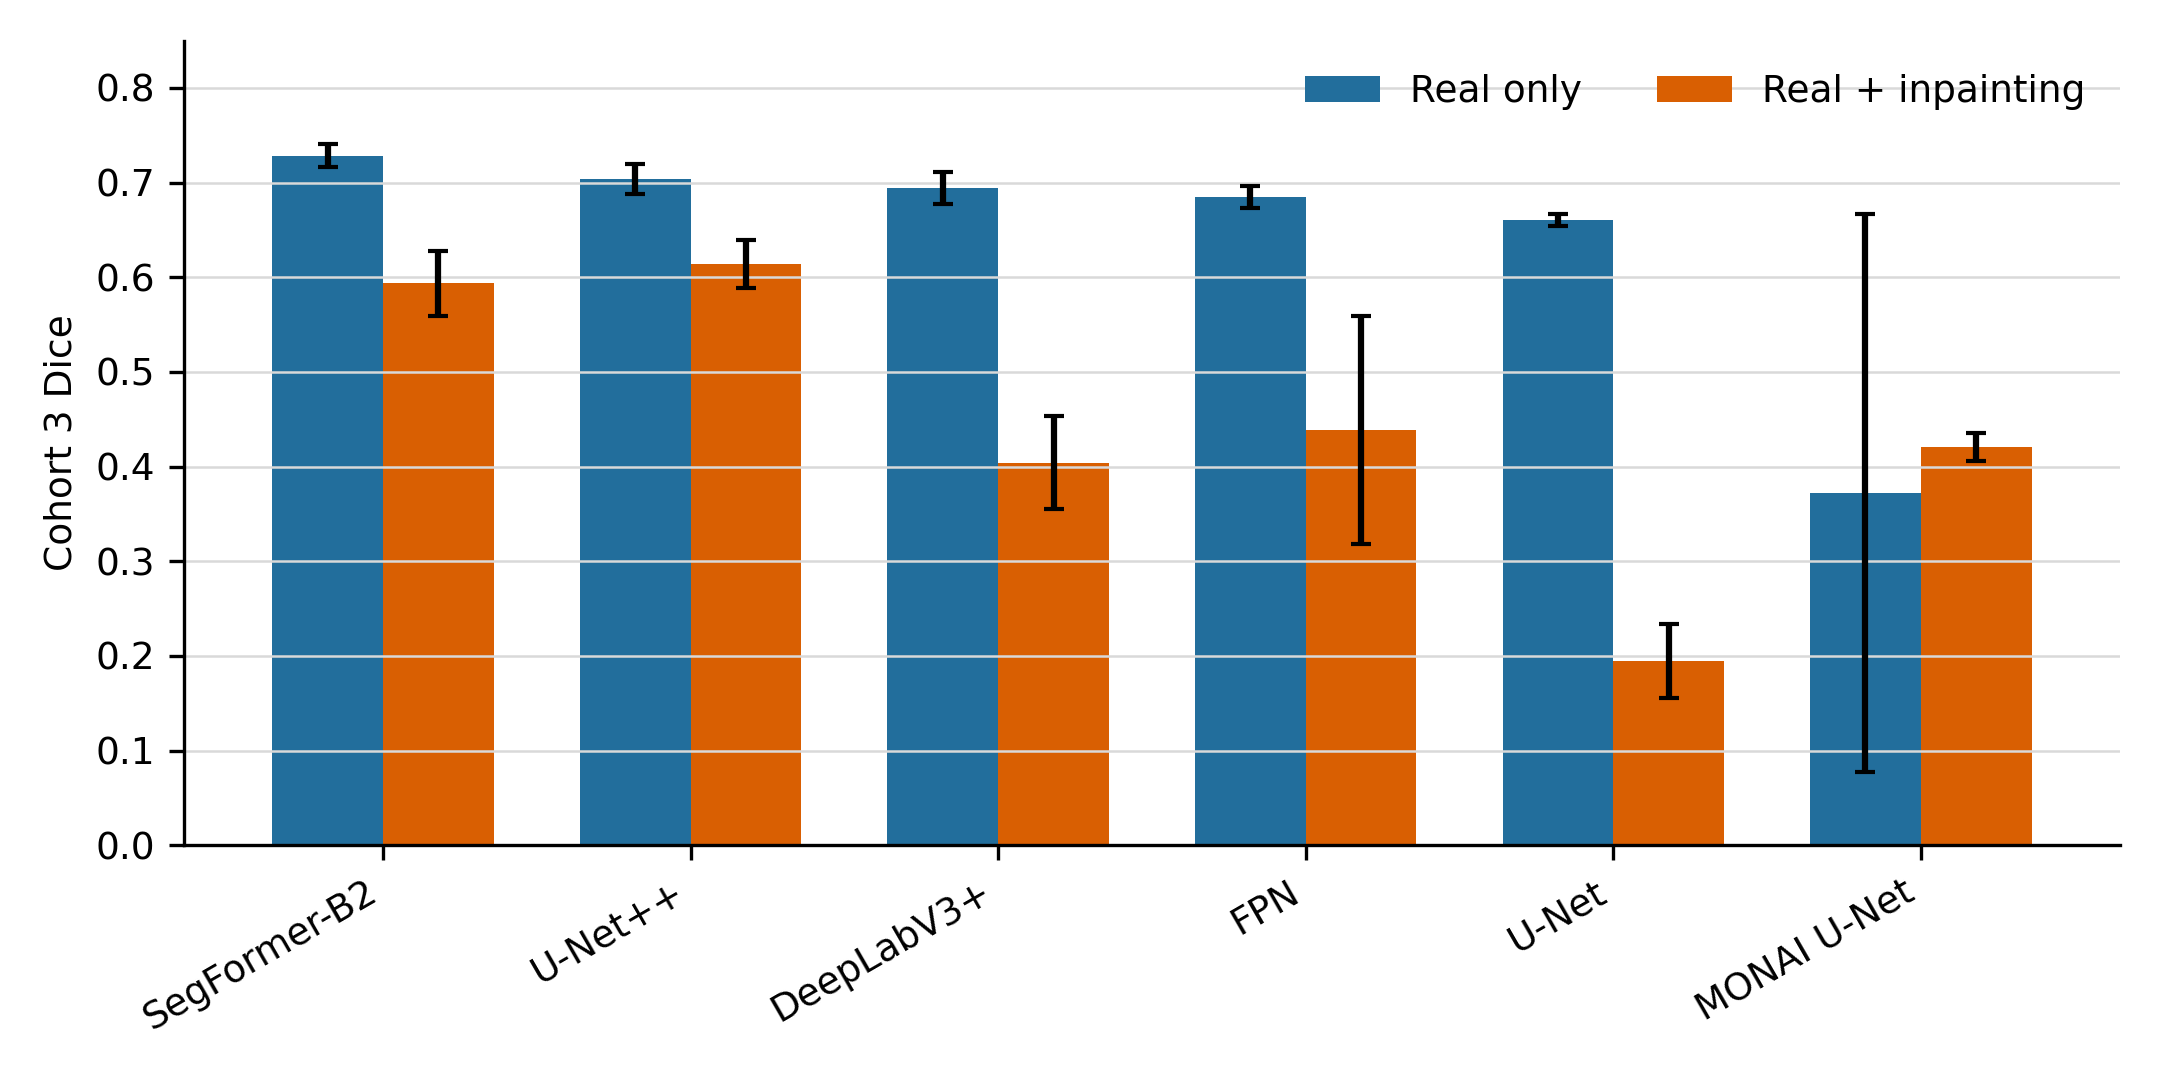
\includegraphics[width=0.94\textwidth]{fig_journal_c3_model_dice.pdf}
  \caption{Held-out Cohort 3 Dice by model and training condition. Bars show mean over three seeds; error bars show standard deviation across seeds. Real-only training outperformed real-plus-inpainting training for every evaluated architecture.}
  \label{fig:model-dice}
\end{figure}

\begin{table}[H]
  \centering
  \caption{Held-out Cohort 3 performance by training condition. Values summarize 18 semantic checkpoints per condition.}
  \label{tab:condition-results}
  \begin{tabular}{lrrrrr}
    \toprule
    \textbf{Training condition} & \textbf{Runs} & \textbf{Dice} & \textbf{IoU} & \textbf{Boundary F1} & \textbf{Best val Dice} \\
    \midrule
    Real only & 18 & 0.641 $\pm$ 0.161 & 0.519 $\pm$ 0.138 & 0.703 & 0.758 \\
    Real + inpainting & 18 & 0.444 $\pm$ 0.151 & 0.345 $\pm$ 0.126 & 0.500 & 0.947 \\
    \bottomrule
  \end{tabular}
\end{table}

Real-only training produced the best condition-level result, with mean Dice 0.641 and mean IoU 0.519 across all six architectures and three seeds. Real-plus-inpainting had substantially lower held-out performance, with mean Dice 0.444 and mean IoU 0.345, despite much higher validation Dice. This indicates that the inpainting validation distribution was not a reliable proxy for ecological test generalization.

\subsection{Model-Level Results}

Model architecture had a large effect on held-out performance (Table~\ref{tab:model-results}). Under real-only training, SegFormer-B2, U-Net++, DeepLabV3+, FPN, and U-Net all produced mean Dice above 0.66. MONAI U-Net was unstable because one seed over-segmented foreground, leading to high recall but poor precision.

\begin{table}[H]
  \centering
  \caption{Held-out Cohort 3 performance by model and condition. Values are mean $\pm$ standard deviation over three seeds.}
  \label{tab:model-results}
  \begin{tabular}{llrrr}
    \toprule
    \textbf{Condition} & \textbf{Model} & \textbf{Dice} & \textbf{IoU} & \textbf{Boundary F1} \\
    \midrule
    Real only & SegFormer-B2 & 0.728 $\pm$ 0.012 & 0.607 $\pm$ 0.011 & 0.795 \\
    Real only & U-Net++ & 0.704 $\pm$ 0.016 & 0.577 $\pm$ 0.016 & 0.776 \\
    Real only & DeepLabV3+ & 0.694 $\pm$ 0.017 & 0.566 $\pm$ 0.016 & 0.763 \\
    Real only & FPN & 0.685 $\pm$ 0.011 & 0.552 $\pm$ 0.012 & 0.757 \\
    Real only & U-Net & 0.660 $\pm$ 0.007 & 0.534 $\pm$ 0.007 & 0.735 \\
    Real only & MONAI U-Net & 0.372 $\pm$ 0.295 & 0.278 $\pm$ 0.227 & 0.390 \\
    \midrule
    Real + inpainting & U-Net++ & 0.614 $\pm$ 0.026 & 0.495 $\pm$ 0.021 & 0.686 \\
    Real + inpainting & SegFormer-B2 & 0.594 $\pm$ 0.034 & 0.468 $\pm$ 0.037 & 0.650 \\
    Real + inpainting & FPN & 0.439 $\pm$ 0.120 & 0.344 $\pm$ 0.101 & 0.500 \\
    Real + inpainting & MONAI U-Net & 0.421 $\pm$ 0.015 & 0.301 $\pm$ 0.009 & 0.473 \\
    Real + inpainting & DeepLabV3+ & 0.404 $\pm$ 0.049 & 0.312 $\pm$ 0.039 & 0.466 \\
    Real + inpainting & U-Net & 0.195 $\pm$ 0.039 & 0.148 $\pm$ 0.030 & 0.223 \\
    \bottomrule
  \end{tabular}
\end{table}

The top eight runs all came from the real-only condition. The best inpainting-assisted models were U-Net++ and SegFormer-B2, but neither exceeded the best real-only checkpoints. This result does not show that synthetic context is intrinsically harmful; rather, it shows that this inpainting pipeline did not improve held-out ecological segmentation under the present training and evaluation protocol.

\subsection{Validation Versus Test Generalization}

The largest scientific signal is the difference between validation and held-out ecological test performance. Real-only models had a mean validation-to-test Dice gap of 0.117. Real-plus-inpainting models had a mean gap of 0.502, indicating that the synthetic validation distribution was much easier than the locked ecological test set.

\begin{figure}[H]
  \centering
  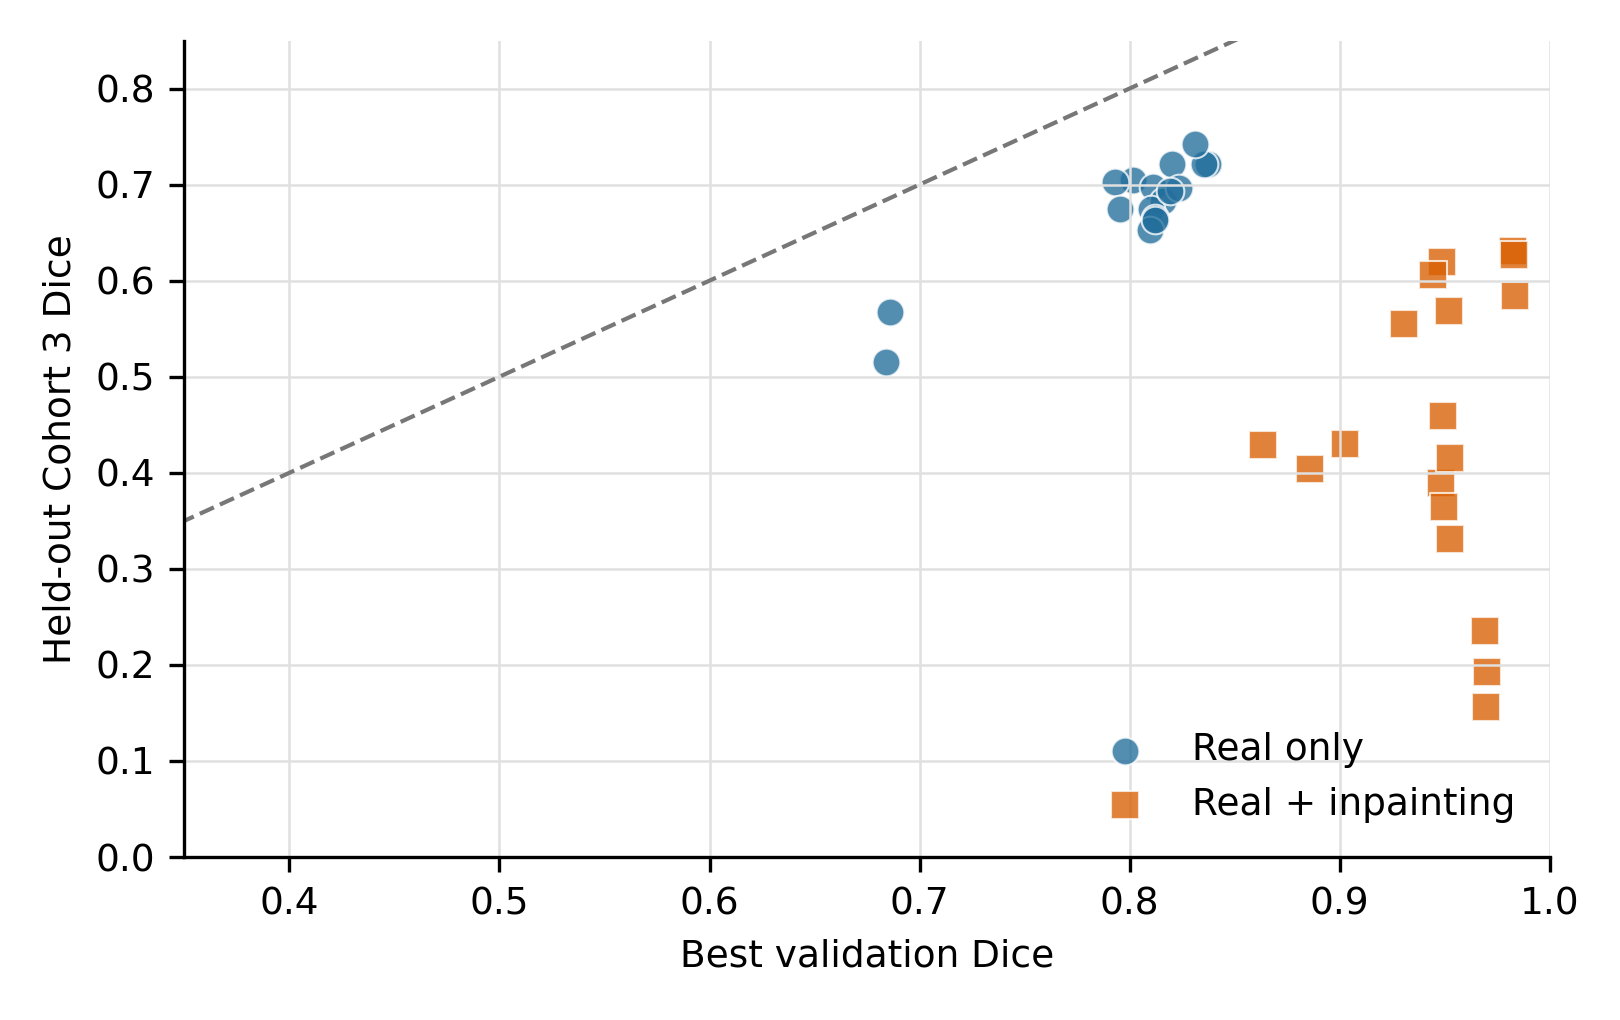
\includegraphics[width=0.72\textwidth]{fig_journal_generalization_gap.pdf}
  \caption{Validation Dice versus held-out Cohort 3 Dice. The dashed line indicates perfect agreement. Real-plus-inpainting checkpoints reached high validation Dice but often failed to transfer to the ecological test set, revealing a substantial synthetic-to-real generalization gap.}
  \label{fig:generalization-gap}
\end{figure}

\subsection{Qualitative Segmentation}

Figure~\ref{fig:qualitative} shows representative predictions from the best completed checkpoint, SegFormer-B2 trained on real images only. The model captures many elongated and irregular microplastic regions while preserving visually complex background context. Remaining errors include partial boundary misses, small false-positive fragments, and difficulty with very faint or transparent foreground.

\begin{figure}[H]
  \centering
  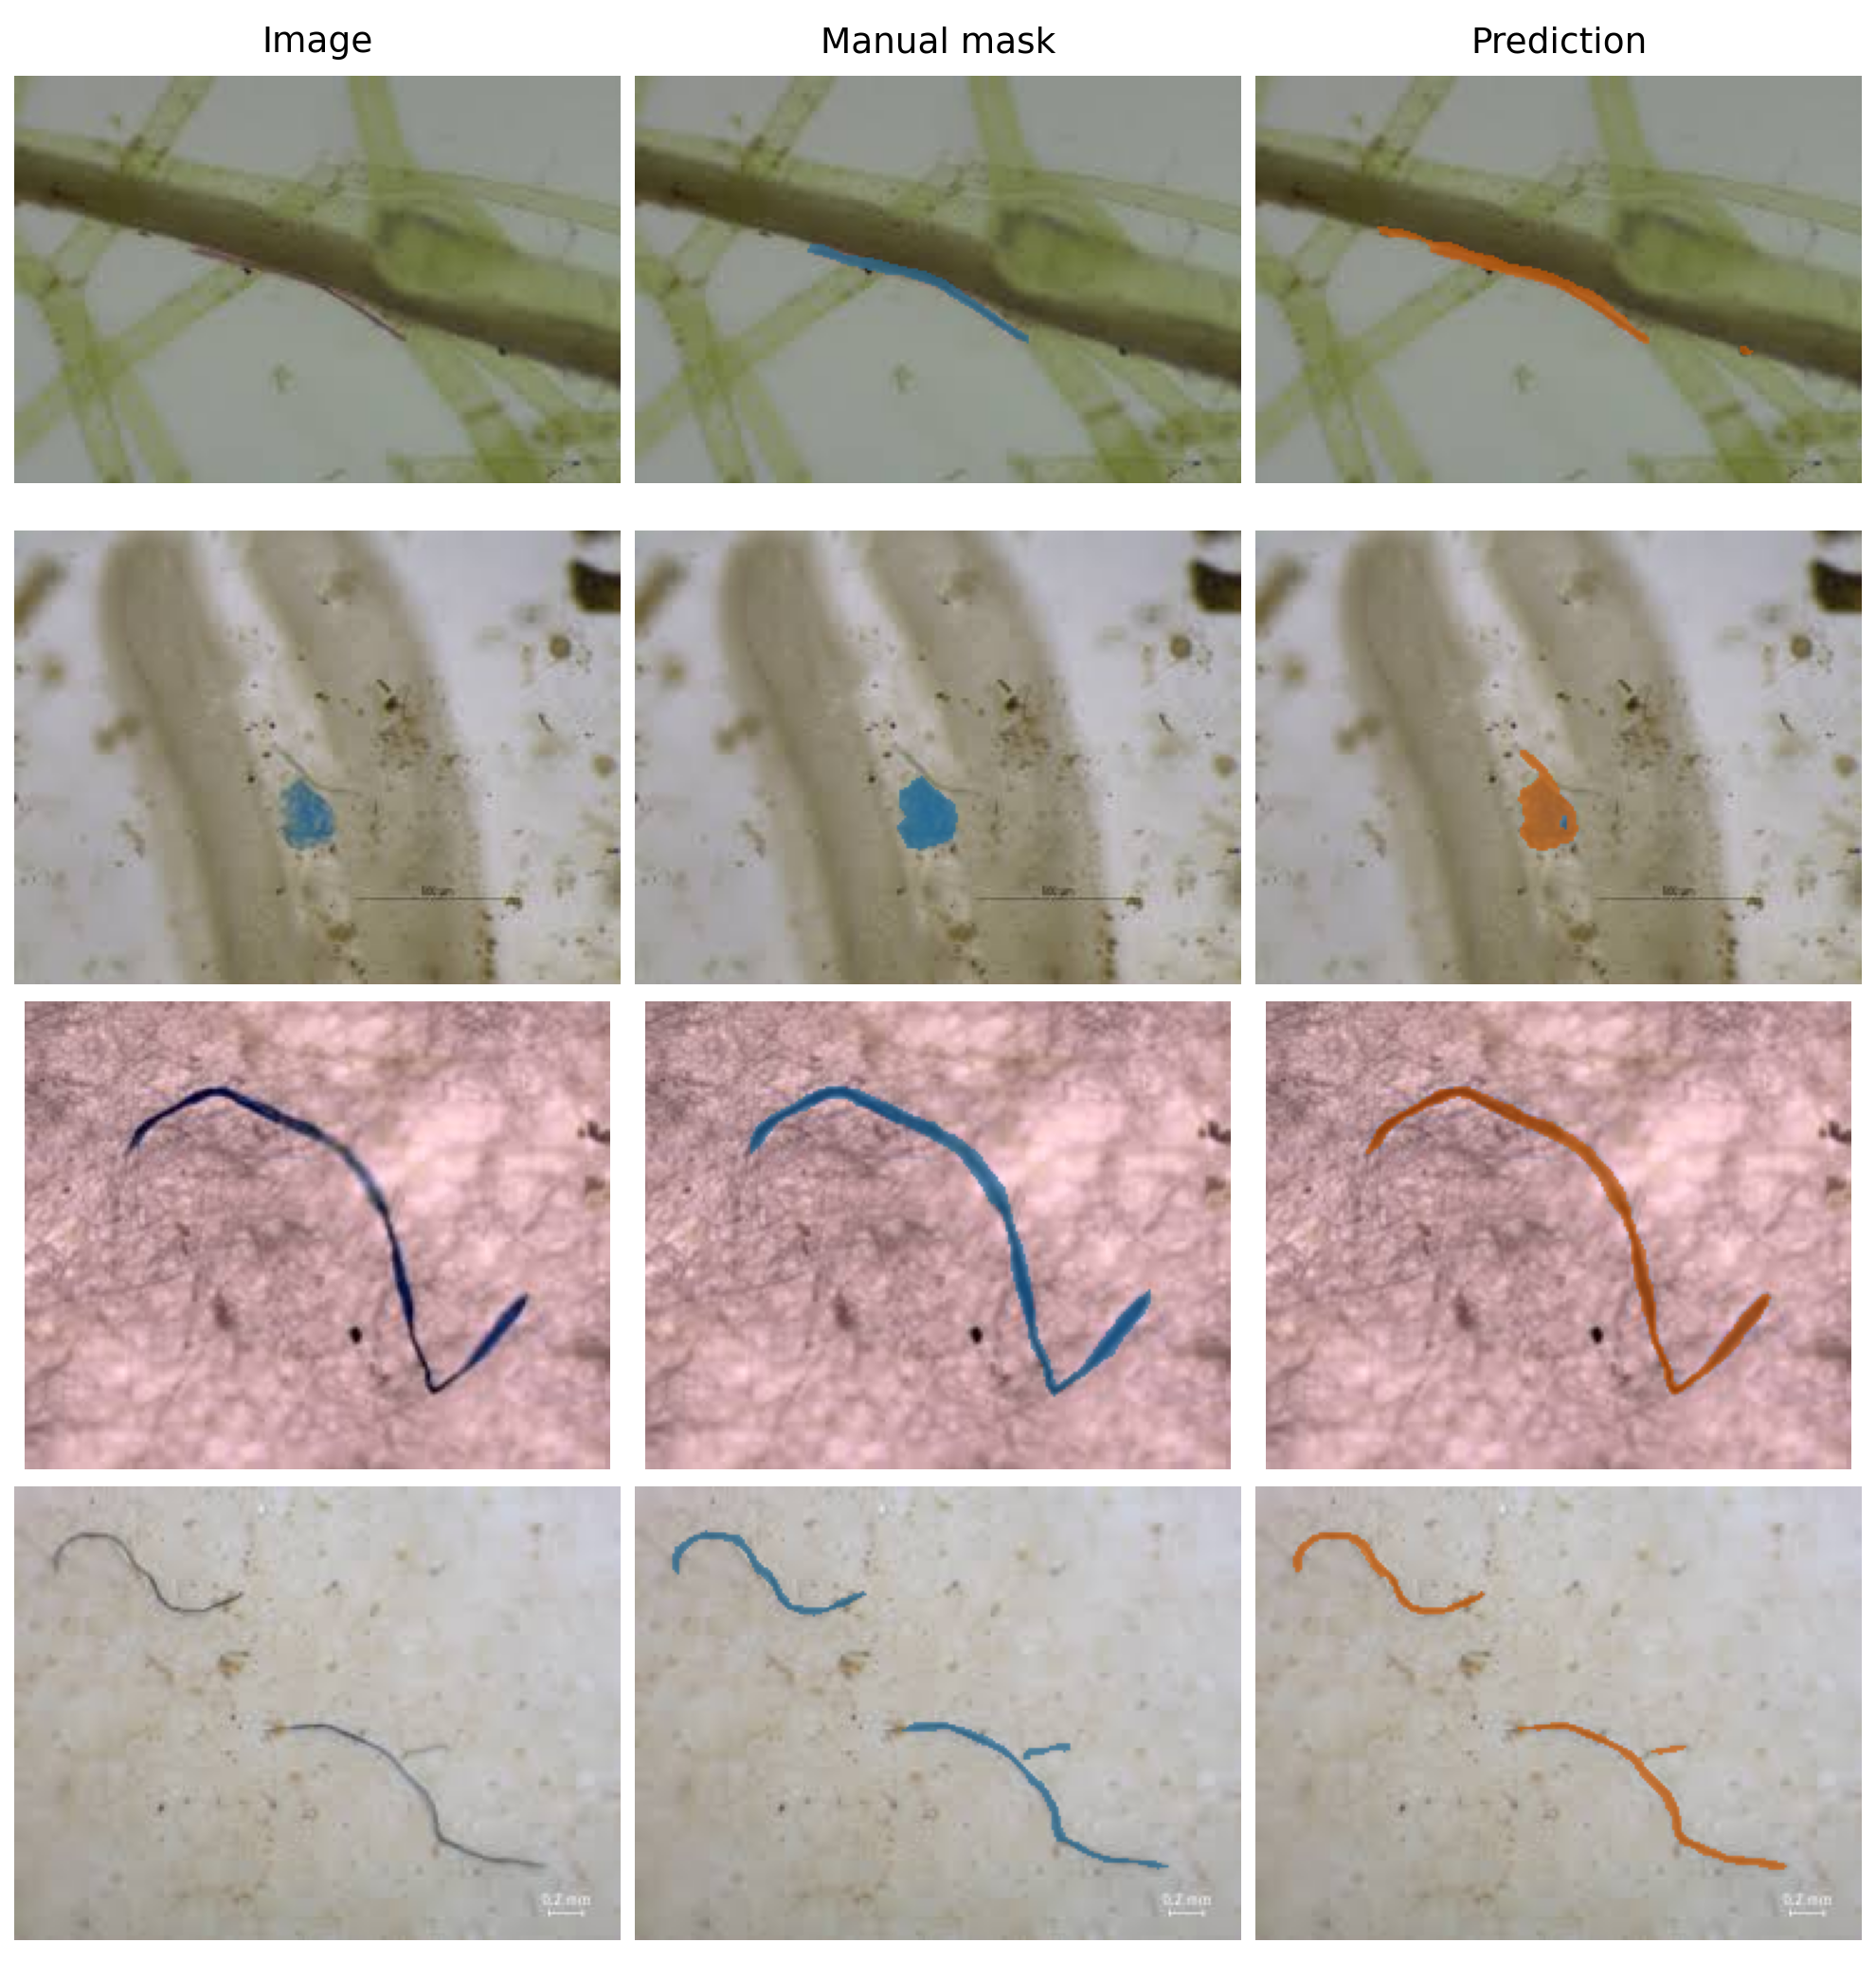
\includegraphics[width=0.9\textwidth]{fig_journal_qualitative_masks.png}
  \caption{Qualitative Cohort 3 examples from the strongest completed checkpoint. Columns show real microscopy image, manual mask overlay, and predicted mask overlay. Blue indicates manual microplastic foreground; orange indicates model-predicted foreground.}
  \label{fig:qualitative}
\end{figure}

\section{Discussion}

The completed results support two practical conclusions. First, deep segmentation models can produce useful ecological microplastic masks from brightfield microscopy images. The best SegFormer-B2 checkpoint achieved Dice 0.743 and IoU 0.619 on a locked ecological test set, with qualitatively coherent masks on cluttered images. These values are lower than some controlled-modality reports in fluorescence or optical micrograph settings \cite{park2022mpnet,hao2024}, but the comparison is not one-to-one: this study evaluates brightfield ecological images with debris, background heterogeneity, and small foreground masks.

Second, synthetic ecological context should be evaluated carefully. The real-plus-inpainting condition produced very high validation Dice, especially for U-Net++, U-Net, FPN, DeepLabV3+, and SegFormer-B2. Yet the same checkpoints performed worse than real-only training on the held-out ecological test set. This gap suggests that the inpainted images created a validation distribution that was visually or statistically easier than real ecological microplastic images. In practical terms, synthetic data should not be accepted as beneficial unless it improves a locked real test set.

The result is useful even though it is not the synthetic-data outcome one might expect. It identifies a strong current baseline for ecological microplastic segmentation and clarifies that inpainting alone is not enough. Future synthetic data work should include stricter visual quality control, generator artifact screening, domain-randomized background selection, prompt ablations, and final evaluation on real ecological images from sites and imaging devices not used during generation.

For deployment, the model should be treated as an image-screening and measurement aid rather than a chemical identifier. A mask can support candidate particle localization, foreground area estimation, morphology measurement, and expert review. Polymer identity still requires confirmatory analysis such as FTIR, Raman spectroscopy, or domain-expert verification when material classification is required.

\section{Limitations}

The Cohort 3 test set contains 97 images, which is sufficient for a controlled benchmark but not sufficient to represent all environmental settings, imaging instruments, sample preparations, or polymer types. The inpainting condition used generated images with retained binary masks, but those masks may not perfectly match the visual boundaries created by the generator. This label-image mismatch may explain part of the generalization gap. Finally, conclusions are limited to the completed semantic segmentation comparison reported here.

\section{Conclusion}

This study provides a focused, completed benchmark for ecological microplastic segmentation. SegFormer-B2 trained on real labeled images only was the strongest model, reaching held-out Dice 0.743 and IoU 0.619. Across six architectures and three seeds, real-only training outperformed real-plus-inpainting training on the locked ecological test set. The results show that professional-quality microplastic segmentation is feasible, while also demonstrating that synthetic validation performance can substantially overstate real ecological generalization. The released metrics, figures, and reproducible training protocol establish a defensible baseline for segmentation-assisted microplastic image screening.

\section*{Data and Code Availability}

The project code and training pipeline are available in the \href{https://github.com/axel-slid/Microplastic-Segmentation-GAN/tree/main}{GitHub repository}. The associated data archive is available through the \href{https://dataverse.harvard.edu/dataverse/Microplastic-Segmentation-GAN/}{Harvard Dataverse microplastic segmentation collection}. All reported metrics in this manuscript are generated from the locked Cohort 3 evaluation files in the project workspace.

\section*{Acknowledgments}

We thank the Moore Institute for Plastic Pollution Research for providing microplastic imagery and supporting data resources used in this work.

\begin{thebibliography}{99}

\bibitem{ziani2023}
Ziani, K. et al. (2023) Microplastics: A real global threat for environment and food safety: A state of the art review. \textit{Nutrients} \textbf{15}(3):617. doi:10.3390/nu15030617.

\bibitem{geyer2017}
Geyer, R., Jambeck, J.R., and Law, K.L. (2017) Production, use, and fate of all plastics ever made. \textit{Science Advances} \textbf{3}:e1700782. doi:10.1126/sciadv.1700782.

\bibitem{hidalgo2012}
Hidalgo-Ruz, V., Gutow, L., Thompson, R., and Thiel, M. (2012) Microplastics in the marine environment: A review of the methods used for identification and quantification. \textit{Environmental Science \& Technology} \textbf{46}:3060--3075. doi:10.1021/es2031505.

\bibitem{stock2020}
Stock, F. et al. (2020) Pitfalls and limitations in microplastic analyses. \textit{Plastics in the Aquatic Environment - Part I. The Handbook of Environmental Chemistry}, vol. 111. Springer, Cham. doi:10.1007/698\_2020\_654.

\bibitem{primpke2020}
Primpke, S., Christiansen, S.H., Cowger, W., et al. (2020) Critical assessment of analytical methods for the harmonized and cost-efficient analysis of microplastics. \textit{Applied Spectroscopy} \textbf{74}(9):1012--1047. doi:10.1177/0003702820921465.

\bibitem{lorenzo2021}
Lorenzo-Navarro, J., Castrill\'on-Santana, M., S\'anchez-Nielsen, E., Zarco, B., Herrera, A., and Mart\'inez, I. (2021) Deep learning approach for automatic microplastics counting and classification. \textit{Science of The Total Environment} \textbf{765}:142728. doi:10.1016/j.scitotenv.2020.142728.

\bibitem{park2022mpnet}
Park, H., Park, S., de Guzman, M.K., Baek, J.Y., Cirkovic Velickovic, T., Van Messem, A., and De Neve, W. (2022) MP-Net: Deep learning-based segmentation for fluorescence microscopy images of microplastics isolated from clams. \textit{PLOS ONE} \textbf{17}(6):e0269449. doi:10.1371/journal.pone.0269449.

\bibitem{shi2022sem}
Shi, B., Patel, M., Yu, D., Yan, J., Li, Z., Petriw, D., Pruyn, T., Smyth, K., Passeport, E., Miller, R.J.D., and Howe, J.Y. (2022) Automatic quantification and classification of microplastics in scanning electron micrographs via deep learning. \textit{Science of The Total Environment} \textbf{825}:153903. doi:10.1016/j.scitotenv.2022.153903.

\bibitem{hao2024}
Hao, Y., Wang, P., Cui, M., Zeng, Z., Ma, S., Li, Y., Zou, T., Fang, X., and Lin, L. (2024) Automatic localization and segmentation of adherent microplastics in optical micrographs based on improved YOLOv5 and adaptive perceptual UNET 3+++. \textit{Biomedical Signal Processing and Control} \textbf{95}:106399. doi:10.1016/j.bspc.2024.106399.

\bibitem{yao2025}
Yao, Y., Xu, W., and Fan, H. (2025) A deep learning approach for microplastic segmentation in microscopic images. \textit{Toxics} \textbf{13}(12):1018. doi:10.3390/toxics13121018.

\bibitem{ronneberger2015}
Ronneberger, O., Fischer, P., and Brox, T. (2015) U-Net: Convolutional networks for biomedical image segmentation. \textit{MICCAI}, 234--241.

\bibitem{zhou2018}
Zhou, Z., Siddiquee, M.M.R., Tajbakhsh, N., and Liang, J. (2018) UNet++: A nested U-Net architecture for medical image segmentation. \textit{Deep Learning in Medical Image Analysis and Multimodal Learning for Clinical Decision Support}, 3--11.

\bibitem{chen2018}
Chen, L.-C., Zhu, Y., Papandreou, G., Schroff, F., and Adam, H. (2018) Encoder-decoder with atrous separable convolution for semantic image segmentation. \textit{ECCV}, 801--818.

\bibitem{lin2017}
Lin, T.-Y., Doll\'ar, P., Girshick, R., He, K., Hariharan, B., and Belongie, S. (2017) Feature pyramid networks for object detection. \textit{CVPR}, 2117--2125.

\bibitem{xie2021}
Xie, E., Wang, W., Yu, Z., Anandkumar, A., Alvarez, J.M., and Luo, P. (2021) SegFormer: Simple and efficient design for semantic segmentation with transformers. \textit{NeurIPS}.

\end{thebibliography}

\end{document}
